\documentclass[12pt]{article}

\usepackage{amscd}
\usepackage{amsmath}
\usepackage{amssymb}
\usepackage{amsthm}
\usepackage{color}
\usepackage{epsfig}
\usepackage{extarrows}
\usepackage{graphicx}
\usepackage{hyperref}
\usepackage{mathrsfs}
\usepackage{mathtools}
\usepackage{verbatim}
\usepackage{tikz}
\usepackage{xypic}
%\usepackage[all,dvips]{xy}

\usetikzlibrary{matrix}

\begin{comment}  

This LaTeX document is a template to be used by Bates mathematics rising seniors to create a thesis proposal. 

As a guide, the document is already filled out to represent a fictitious proposal, and all you need to do is modify the entries below to represent your own proposal.

A PDF version of the fictitious proposal is available on the department's FAQ and Policies pages, at
                   http://abacus.bates.edu/acad/depts/math/faq.html
      and
                   http://abacus.bates.edu/acad/depts/math/policies.html
      respectively.

Once you have finished your proposal, export it to a PDF file. Give the file a USEFUL name, for example, RiemannThesisProposal.PDF. Email the PDF file to Clementine Brasier, the 
Academic Administrative Assistant for Hathorn Hall, at cbrasier\@bates.edu

                This LaTex document was created Feb/Mar 2010 by Adriana Salerno and updated Feb 2012 by Meredith Greer

\end{comment}

\setlength{\textheight}{8.5in} \setlength{\topmargin}{0.0in}
\setlength{\headheight}{0.0in} \setlength{\headsep}{0.0in}
\setlength{\leftmargin}{0.5in}
\setlength{\oddsidemargin}{0.0in}
%\setlength{\parindent}{1pc}
\setlength{\textwidth}{6.5in}
%\linespread{1.6}

\newtheorem{conjecture}{Conjecture}
\newtheorem*{conjecture*}{Conjecture}

\newtheorem{corollary}{Corollary}
\newtheorem*{corollary*}{Corollary}

\newtheorem{definition}{Definition}
\newtheorem*{definition*}{Definition}

\newtheorem{example}{Example}
\newtheorem*{example*}{Example}

\newtheorem{lemma}{Lemma}
\newtheorem*{lemma*}{Lemma}

\newtheorem{note}{Note}
\newtheorem*{note*}{Note}

\newtheorem{problem}{Problem}
\newtheorem*{problem*}{Problem}

\newtheorem{prop}{Proposition}
\newtheorem*{prop*}{Proposition}

\newtheorem{question}{Question}
\newtheorem*{question*}{Question}

\newtheorem{theorem}{Theorem}
\newtheorem*{theorem*}{Theorem}

%%%%%%%%%%%%%%%%%%%%%%%%%%%%%%%%%%%%%%%%%

\begin{document}

\title{K-theory, Chern-Connes Character and Algebraic Novikov Conjecture}
\author{Yihan Zhang}
\maketitle

\tableofcontents
\bigskip

\section{K-theory}
Recall history of K-theory.
\begin{enumerate}
	\item Grothendieck, Riemann-Roch Theorem(for algebraic variety).
	\item Atiyah, Hirzebruch, topological K-theory.
	\item Quillen, Milnor, Bass, algebraic K-theory.
\end{enumerate}
Applications: topology, operator algebra, algebra, number theory, etc.

$R$, a unital ring. $M_n(R)=\left\{\left(\begin{array}{ccc} r_{11} & \cdots & r_{1n} \\ & \cdots & \\ r_{n1} & \cdots & r_{nn} \end{array}\right): r_{ij}\in R \right\}. $ $M_\infty(R)=\bigcup_{n=1}^\infty M_n(R) $. $M_n(R)\xhookrightarrow[]{} M_{n+1}(R), \left(\begin{array}{ccc}r_{11}&\cdots&r_{1n}\\&\cdots&\\r_{n1}&\cdots&r_{nn} \end{array} \right)\to \left(\begin{array}{cccc}r_{11}&\cdots&r_{1n}&0\\\cdots&\cdots&\cdots&\cdots\\r_{n1}&\cdots&r_{nn}&0\\0&\cdots&\cdots&0 \end{array} \right).$ Idempotent $p\in M_\infty(R)$, $p^2=p$.
\begin{example}
$X$, a compact space. $R=C(X)$. Idempotent $p\in M_\infty(C(X)) \iff $ vector bundle over $X$. $p:X\to M_n(\mathbb C),x\mapsto p(x)$.
\end{example}
$Idempotent(M_\infty(R))/\sim$, abelian semigroup. Two idempotents $p,q$ are said to be equivalent if $\exists$ an invertible $w\in M_n(R)$ s.t. $w^{-1}pw=q$. $[p]+[q]=\left[\left(\begin{array}{cc}p&0\\0&q \end{array} \right) \right]$. Notice that $\left(\begin{array}{cc}0&1\\1&0 \end{array} \right)^{-1}\left(\begin{array}{cc}p&0\\0&q \end{array} \right)\left(\begin{array}{cc}0&1\\1&0 \end{array} \right)=\left(\begin{array}{cc}q&0\\0&p \end{array} \right). $

$S$(abelian semigroup)$\xrightarrow[]{\text{Grothendieck process}}$$G(S)$(abelian group). $G(s)=\{(s,t):s,t\in S \}/\sim$. $(s,t)\sim(s',t') $ iff $\exists x\in S $ s.t. $s+t'+x=s'+t+x$. $-[(s,t)]=[(t,s)]$.
\begin{example}
$S=\mathbb N,G(s)=\mathbb Z$.
\end{example}
\begin{example}
$S=\mathbb N\cup\{+\infty\},G(S)=\{0\}$. Notice that $(s,t)\sim(s',t'),s+t'+\infty=s'+t+\infty $.
\end{example}
\begin{definition}
$K_0(R)=G(Idempotent(M_\infty(R))/\sim)$.
\end{definition}
$\Gamma$, a group. Group ring, $\mathbb C\Gamma=\left\{\sum_{g\in\Gamma}c_gg:c_g\in\mathbb C \right\}$, where elements are finite sum. $U_g:\ell^2(\Gamma)\to \ell^2(\Gamma)$, $(U_g\xi)(x)=\xi(g^{-1}x)$. Then $\mathbb C\Gamma=\left\{\sum_{g\in\Gamma}c_gU_g \right\}\subset \mathcal B(\ell^2(\Gamma))$.

$R$, a ring. Group ring, $R\Gamma=\left\{\sum_{g\in\Gamma}r_gg:r_g\in R \right\}$. Question: what is $K_0(R\Gamma)$?

\section{Chern-Connes Character}
$\forall p\ge 1, T:H\to H$ is called a Schatten $p$-class operator if $tr(T^*T)^{\frac{p}{2}}<+\infty$. $T=diag(c_1,\cdots,c_n,\cdots)$, $tr(T^*T)^{\frac{p}{2}}=\sum_{n=1}^\infty|c_n|^p<+\infty$.
\begin{definition}
$S_p$, the ring of all Schatten $p$-class operators. $S=\bigcup_{p=1}^\infty S_p$, the ring of all Schatten class operators.
\end{definition}
$\Gamma$, a group. $S$, the ring of Schatten class operators. $S\Gamma$, the group ring. Motivations: Connes-Moscovici's higher index theory(1990s, \textit{Topology}). $M^{2n}$, a compact manifold. $D$, an elliptic differential operator on $M^{2n}$. Higher index, index $D\in K_0(S\Gamma)$, $\Gamma=\pi_1M$.

Approximating $K_0(S\Gamma)$ using locally finite simplicial homology group of $P_F(\Gamma)$. $\Gamma$, a group. $\forall F\subset \Gamma$, a finite subset.
\begin{definition}
The Rips' complex $P_F(\Gamma)$ is a simplicial complex whose set of vertices is $\Gamma$ and $\{\gamma_0,\cdots,\gamma_n\}$ spans a simplex iff $\gamma_i^{-1}\gamma_j\in F$.
\end{definition}
\begin{example}
$\Gamma=\mathbb Z$. $F=\{\pm 1\}$. $\{n_0,n_1\}$ spans a simplex. $n_1-n_0\in F=\{\pm1\}$. $P_F(\Gamma)$ forms a line.
\end{example}
\begin{example}
$\Gamma=\mathbb F_2=<a,b>$. $F=\{a^{\pm1},b^{\pm1} \}$. $\gamma_0^{-1}\gamma_1\in F$. $P_F(\Gamma)$ forms a tree.
\end{example}
$X$, a simplicial complex. $H_*^{lf}(X)$, the locally finite homology group of $X$. $C_n^{lf}(X)$, the $n$-dimensional locally finite simplicial chain group. $C_n^{lf}(X)=\left\{\sum c_{[v_0,\cdots,v_n]}[v_0,\cdots,v_n]:c_{[v_0,\cdots,v_n]}\in \mathbb C \right\}$. $[v_0,\cdots,v_n]$, oriented simplex with vertices $v_0,\cdots,v_n$. $\sum c_{[v_0,\cdots,v_n]}[v_0,\cdots,v_n]$ locally finite, i.e. $\forall$ a compact subset $K\subset X$, $\exists$ at most finitely many $[v_0,\cdots,v_n]$ s.t. $c_{[v_0,\cdots,v_n]}\ne 0$ and $[v_0,\cdots,v_n]\cap K\ne \phi$. $\partial_n:C_n^{lf}(X)\to C_{n-1}^{lf}(X)$, boundary map. $\partial_n[v_0,\cdots,v_n]=\sum_{i=0}^n(-1)^i[v_0,\cdots,\hat{v_i},\cdots,v_n]$.
\begin{definition}
$H_n^{lf}(X)=Ker\partial_n/Im\partial_{n+1}$.
\end{definition}
\begin{example}
$X=\mathbb R$. $H_1^{lf}(\mathbb R)=\mathbb C$. $H_1(\mathbb R)=0$. Generator of $H_1^{lf}(\mathbb R)$, $\sum_{n=-\infty}^\infty[n,n+1]\in C_1^{lf}(\mathbb R)$. $\partial_1\left(\sum_{n=-\infty}^\infty[n,n+1] \right)=\sum_{n=-\infty}^\infty([n+1]-[n])=0$.
\end{example}
$(v_0,v_1,\cdots,v_n)$, an ordered simplex of $X$($v_i$ may be the same as $v_j$). $(v_0,v_1,\cdots,v_n)\to(v_n,v_0,\cdots,v_{n-1})$ is called a cyclic permutation. $(v_0,\cdots,v_n)\sim(v_0',\cdots,v_n')$ 1. if one can be obtained by any number of cyclic permutations if $n$ is even; 2. one can be obtained from another by even number of cyclic permutation if $n$ is odd. The cyclically oriented simplex $[v_0,\cdots,v_n]_\lambda$ is defined to be the equivalence class of ordered simplex.
\begin{theorem}
$H_{n,\lambda}^{lf}(X)\cong\bigoplus\limits_{\substack{k\le n,\\n-k\ even}}H_k^{lf}(X).$
\end{theorem}
\begin{proof}
$H_{n-2}^{lf}(X)\xhookrightarrow[]{}H_{n,\lambda}^{lf}(X)$. $\sum c_{[v_0,\cdots,v_{n-2}]}[v_0,\cdots,v_{n-2}]\to\sum c_{[v_0,\cdots,v_{n-2}]}[v_0,v_0,v_0,\cdots,v_{n-2}]_\lambda$.
\end{proof}
$\Gamma$, a group. $X$, a simplicial complex. $\Gamma$ acts on $X$ simplicially. Define $H_k^\Gamma(X),H_{k,\lambda}^\Gamma(X)$ by requiring all chains to be $\Gamma$-invariant.

$\Gamma$, a group(torsion free, i.e. if $g^n=1$ for some $g\in \Gamma$, then $n=0$ or $g=1$.). $S$, the ring of Schatten class operators. $c:K_0(S\Gamma)\to\lim\limits_{\substack{finite\ subsets\ F\ of\ \Gamma,\\n\to\infty}}H_{2n,\lambda}^\Gamma(P_F(\Gamma))=\lim\limits_F\left(\bigoplus H_{2k}^\Gamma(P_F(\Gamma)) \right)$. $[p]-[p_0]\in K_0(S_p\Gamma)$ for some $p$. $p\in M_\infty((S_p\Gamma)^+),p_0\in M_\infty(\mathbb C)$ are idempotents. $p=q+p_0,q\in M_\infty(S_p\Gamma)$. Let $q=\sum_{g\in\Gamma}k_gg,k_g\in M_\infty(S_p)$. $c([p]-[p_0])=\sum tr(k_{x_0^{-1}x_1}k_{x_1^{-1}x_2}\cdots k_{x_n^{-1}x_b})[x_0,\cdots,x_n]_\lambda$, where $n\ge p$, $n$ even. Let $F=\{g:k_g\ne0 \}$.
\begin{prop}
$c([p]-[p_0])\in H_n^\Gamma(P_F(\Gamma)).$
\end{prop}

\section{Algebraic K-theory and Novikov Conjecture}
\begin{conjecture}[Novikov]
$\lim\limits_F H_n^\Gamma(P_F(\Gamma), \mathbb K(S)^{-\infty})\xrightarrow[]{assembly\ map} K_n(S\Gamma)$ is rationally injective.
\end{conjecture}
\begin{theorem}
This conjecture is true!
\end{theorem}
\begin{proof}
\[
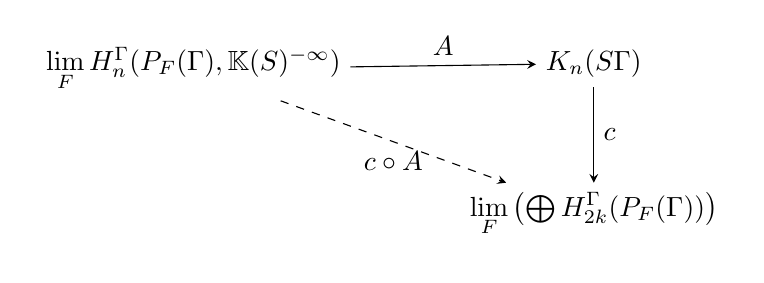
\begin{tikzpicture}
  \matrix (m) [matrix of math nodes,row sep=3em,column sep=4em,minimum width=2em] {
     \lim\limits_F H_n^\Gamma(P_F(\Gamma), \mathbb K(S)^{-\infty}) & K_n(S\Gamma) \\
     & \lim\limits_F\left(\bigoplus H_{2k}^\Gamma(P_F(\Gamma)) \right) \\ 
  };
  \path[-stealth]
    (m-1-1) edge node [above] {$A$} (m-1-2)
    (m-1-2) edge node [right] {$c$} (m-2-2)
    (m-1-1) edge [dashed] node [below] {$c\circ A$} (m-2-2);
\end{tikzpicture}
\]
Claim: $c\circ A$ is rationally an isomorphism(Mayer-Vietoris sequence \& Five Lemma).
\end{proof}

% \begin{thebibliography}{99}
% NOTE: change the "9" above to "99" if you have MORE THAN 10 references.

% \bibitem{erdos1} Erd\"{o}s, P. (1973). Problems and results on combinatorial number theory \uppercase\expandafter{\romannumeral 1}. In \textit{A survey of combinatorial theory (Proc. Internat. Sympos., Colorado State Univ., Fort Collins, Colo., 1971)} (pp. 117-138).

% \end{thebibliography}

%%%%%%%%%%%%%%%%%%%%%%%%%%%%%%%%%%%%%%%%%

\end{document} 
